\documentclass[12pt]{ctexart}
\usepackage[english]{babel} 
\usepackage{fullpage,mathpazo,amsfonts,nicefrac}
\usepackage{mathtools,amssymb}

\newcommand{\N}{\mathbb{N}}
\newcommand{\Z}{\mathbb{Z}}
\newcommand{\Q}{\mathbb{Q}}
\newcommand{\R}{\mathbb{R}}
\newcommand{\norm}[1]{\left\lVert#1\right\rVert} % norm: double vertical bars

\title{	
\normalfont \normalsize 
\huge PRML Homework 1\\ % The assignment title
}

\author{Hao Chen (904547539)} % Your university, school and/or department name(s)

\begin{document}

\maketitle

%\section*{EE236A: Homework 1}
\section{Problem 1}
\begin{enumerate}
\item 
Solution: 
$g_i(x)  = \sum_{y=j} \lambda(\alpha(x)=i | y=j)p(x|y=j)p(y=j)$. \\
As three class models $p(x|y=1), p(x|y=2), p(x|y=3)$ are supposed to be 2D Gaussian distributions with the same covariance matrix $\Sigma=9I$. \\
Thus, 
$\left\{
  \begin{array}{ll}
    p(x | y=1)&= \frac{1}{18\pi} \exp\{-\frac{(x_1-4)^2+(x_2-12)^2}{18}\} \\
    p(x | y=2)&= \frac{1}{18\pi}  \exp\{-\frac{(x_1-12)^2+(x_2-3)^2}{18}\} \\
    p(x | y=3)&= \frac{1}{18\pi}  \exp\{-\frac{(x_1-3)^2+(x_2-5)^2}{18}\} \\
  \end{array}
\right.$ \\
Then, 
$\left\{
  \begin{array}{ll}
    g_1(x)&= \frac{1}{15\pi}  \exp\{-\frac{(x_1-12)^2+(x_2-3)^2}{18}\} + \frac{1}{45\pi}  \exp\{-\frac{(x_1-3)^2+(x_2-5)^2}{18}\}  \\
    g_2(x)&= \frac{2}{45\pi} \exp\{-\frac{(x_1-4)^2+(x_2-12)^2}{18}\} + \frac{1}{90\pi}  \exp\{-\frac{(x_1-3)^2+(x_2-5)^2}{18}\} \\
    g_3(x)&= \frac{1}{15\pi} \exp\{-\frac{(x_1-4)^2+(x_2-12)^2}{18}\} + \frac{1}{45\pi}  \exp\{-\frac{(x_1-12)^2+(x_2-3)^2}{18}\}
  \end{array} 
\right. $ \\

\item 
Solve the $g_i(x) = g_j(x)$ by MATLAB and draw the boundary as following figure. \\
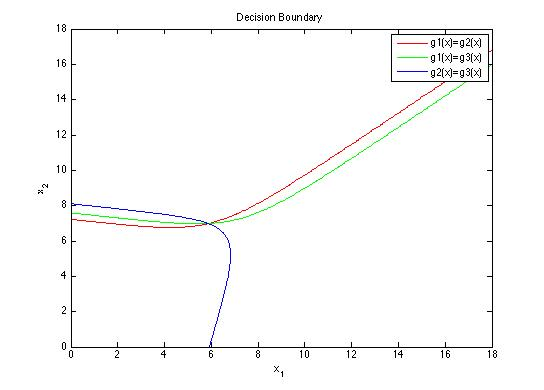
\includegraphics[scale=0.8]{hw1_prob1_pic1.jpg} \\

\item 
When the prior distributions change, the discriminant functions change to: \\
$\left\{
  \begin{array}{ll}
    g_1(x)&= \frac{1}{30\pi}  \exp\{-\frac{(x_1-12)^2+(x_2-3)^2}{18}\} + \frac{1}{15\pi}  \exp\{-\frac{(x_1-3)^2+(x_2-5)^2}{18}\}  \\
    g_2(x)&= \frac{1}{45\pi} \exp\{-\frac{(x_1-4)^2+(x_2-12)^2}{18}\} + \frac{1}{30\pi}  \exp\{-\frac{(x_1-3)^2+(x_2-5)^2}{18}\} \\
    g_3(x)&= \frac{1}{30\pi} \exp\{-\frac{(x_1-4)^2+(x_2-12)^2}{18}\} + \frac{1}{90\pi}  \exp\{-\frac{(x_1-12)^2+(x_2-3)^2}{18}\}
  \end{array} 
\right. $ \\
We re-draw the decision boundary: \\ 
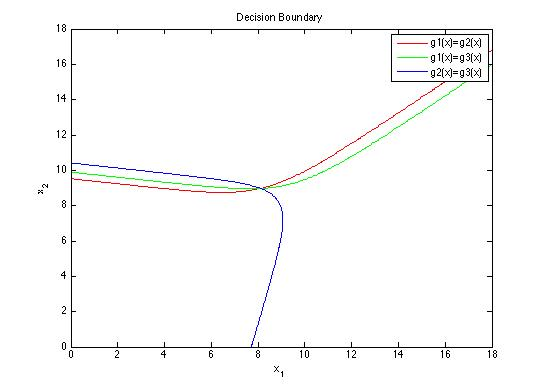
\includegraphics[scale=0.8]{hw1_prob1_pic2.jpg} \\
\end{enumerate}

\section{Problem 2}
\begin{enumerate}
\item Solution
\begin{eqnarray*}
R_{ran} &=& \int_{\Omega^d}  R(\alpha|x)p(x) \mathrm{d}x. \\
	     &=& \int_{\Omega^d} \sum_{j\in \Sigma^c} \lambda(\alpha | y=j) p(y=j|x) p(x)  \mathrm{d}x.  
\end{eqnarray*}
Due to it is 0-1 loss function, and the decision is made by a randomized decision rule, which decides x to class i following $\alpha(x) = y \sim p(y|x)$, so \\
\begin{eqnarray*}
\lambda(\alpha | y=j) &=& \sum_{k \in  \Omega^c, k \neq j} p(\alpha = k) \\
	      		        &=& \sum_{k \in  \Omega^c, k \neq j} p(y = k|x) \\
			        &=& 1 - p(y = j | x) 
\end{eqnarray*}
which leads to
\begin{eqnarray*}
R_{ran} &=& \int_{\Omega^d} \sum_{j\in \Omega^c} (1 - p(y = j | x))p(y=j|x) p(x)  \mathrm{d}x. \\
	     &=& \int_{\Omega^d} (1 - \sum_{j\in \Omega^c} p^2(y=j |x)) p(x) \mathrm{d}x.
\end{eqnarray*}

\item
Proof. 
\begin{eqnarray*}
R_{bayes} &=& \int_{\Omega^d}  R(\alpha|x)p(x) \mathrm{d}x. \\
		 &=& \int_{\Omega^d} (1 - p(y = t|x)) p(x) \mathrm{d}x.  \\
where~~t &=&argmax_{t \in \Omega^c}~~p(y|x).
\end{eqnarray*}

Compare integral parts of $R_{ran}, R_{hayes}$. Now, we consider each possible $x \in \Omega^d$, we want to prove $(1 - p(y = t|x)) p(x) \leq (1 - \sum_{j\in \Omega^c} p^2(y=j |x)) p(x)~~(t =argmax_{t \in \Omega^c}~~p(y|x))$, which can lead to $R_{ran}$ is always larger than or equal to $R_{bayes}$.  
\begin{eqnarray*}
& &(1 - \sum_{j\in \Omega^c} p^2(y=j |x)) - (1 - p(y = t|x)) \\
& = & p(y=t|x) -  \sum_{j\in \Omega^c} p^2(y=j |x) \\
& = & p(y=t|x)(1 - p(y=t|x)) - \sum_{j\in \Omega^c, j \neq t} p^2(y=j |x) \\
& = & p(y=t|x)\sum_{j\in \Omega^c, j \neq t} p(y=j|x) - \sum_{j\in \Omega^c, j \neq t} p^2(y=j |x) \\ 
& = & \sum_{j\in \Omega^c, j \neq t} p(y=j|x) \sum_{j\in \Omega^c, j \neq t} (p(y = t |x) - p(y=j|x)) 
\end{eqnarray*}
Due to $t =argmax_{t \in \Omega^c} p(y|x)$, $(p(y = t |x) - p(y=j|x)) > 0$, which leads to $\sum_{j\in \Omega^c, j \neq t} p(y=j|x) \sum_{j\in \Omega^c, j \neq t} (p(y = t |x) - p(y=j|x)) \geq 0$. Therefore $R_{ran}$ is always larger than or equal to $R_{hayes}$. 

\item 
As we can see the equation in (2), when $p(y = t | x) = p(y = j| x), \forall j \in \Omega^c$, the $R_{ran} = R_{hayes}$, which means that all $p(y = j|x)$ are the same value $= \frac{1}{|\Omega^c|}$.
\end{enumerate}

\section{Problem 3}

\begin{eqnarray*}
p(y = +1|x) &=& \frac{p(x|y= +1) p(y=+1)}{f(x)} \\
		 &=& \frac{p(x|y=+1)p(y=+1)}{p(x|y=+1)p(y=+1) + p(x|y=-1)p(y=-1)} \\ 
\\
p(y = -1|x) &=& \frac{p(x|y=-1)p(y=-1)}{p(x|y=+1)p(y=+1) + p(x|y=-1)p(y=-1)} \\ 
\end{eqnarray*}

plot in MATLAB: \\
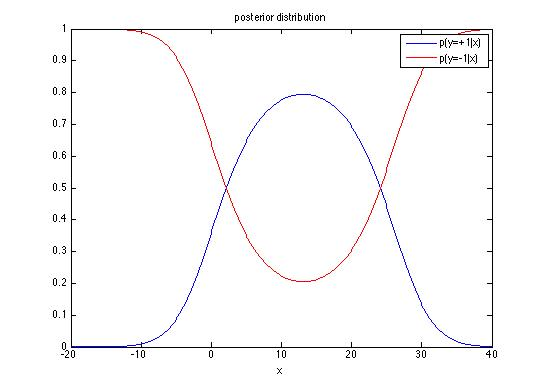
\includegraphics[scale=0.8]{hw1_prob3_pic1.jpg} \\

The ROC and PR curves are showing as: \\
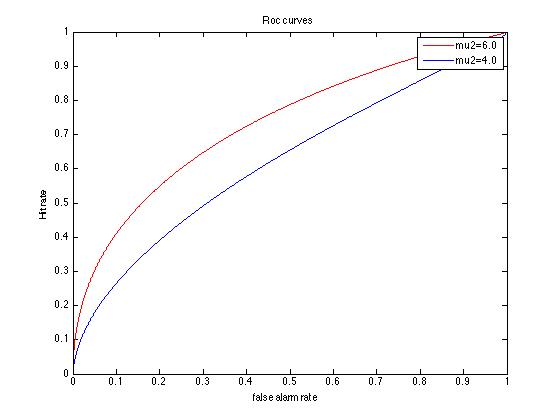
\includegraphics[scale=0.8]{hw1_Roc_curve.jpg} \\
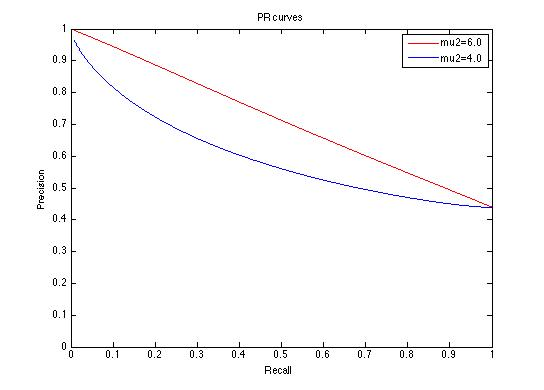
\includegraphics[scale=0.8]{hw1_PR_curve.jpg} \\

\end{document}
